\chapter{Introduction}
\label{ch:introduction}

Welcome to the Duq User Manual. Duq is a powerful envelope-based modulation plugin designed for modern music production.

\section{Overview}
Duq allows you to create complex, multi-point envelopes to modulate various parameters in your DAW. With its intuitive interface and flexible routing, it provides a high degree of control over your sound.

\begin{figure}[h]
    \centering
    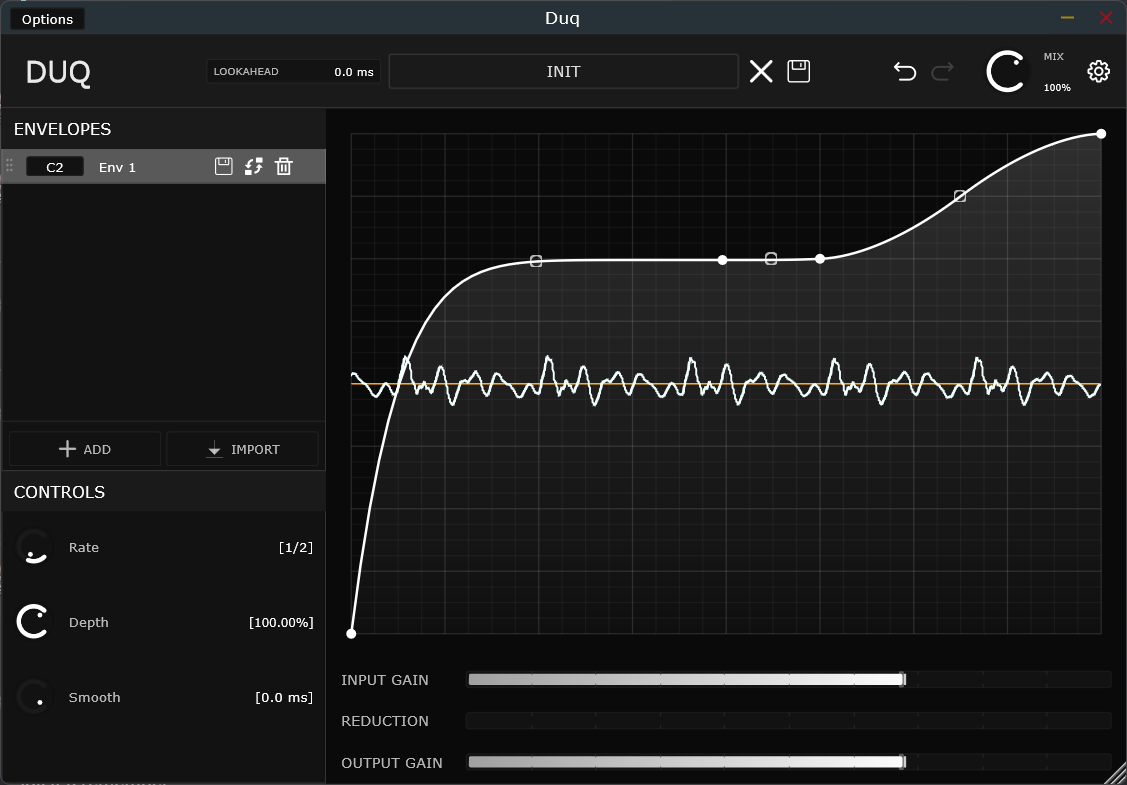
\includegraphics[width=0.8\textwidth]{figures/screenshot1.png}
    \caption{The Duq Main Interface}
    \label{fig:main_interface}
\end{figure}

\section{Key Features}
\begin{itemize}
    \item Multi-point envelope editing.
    \item Real-time visual feedback.
    \item Seamless DAW integration.
\end{itemize}

\begin{figure}[h]
    \centering
    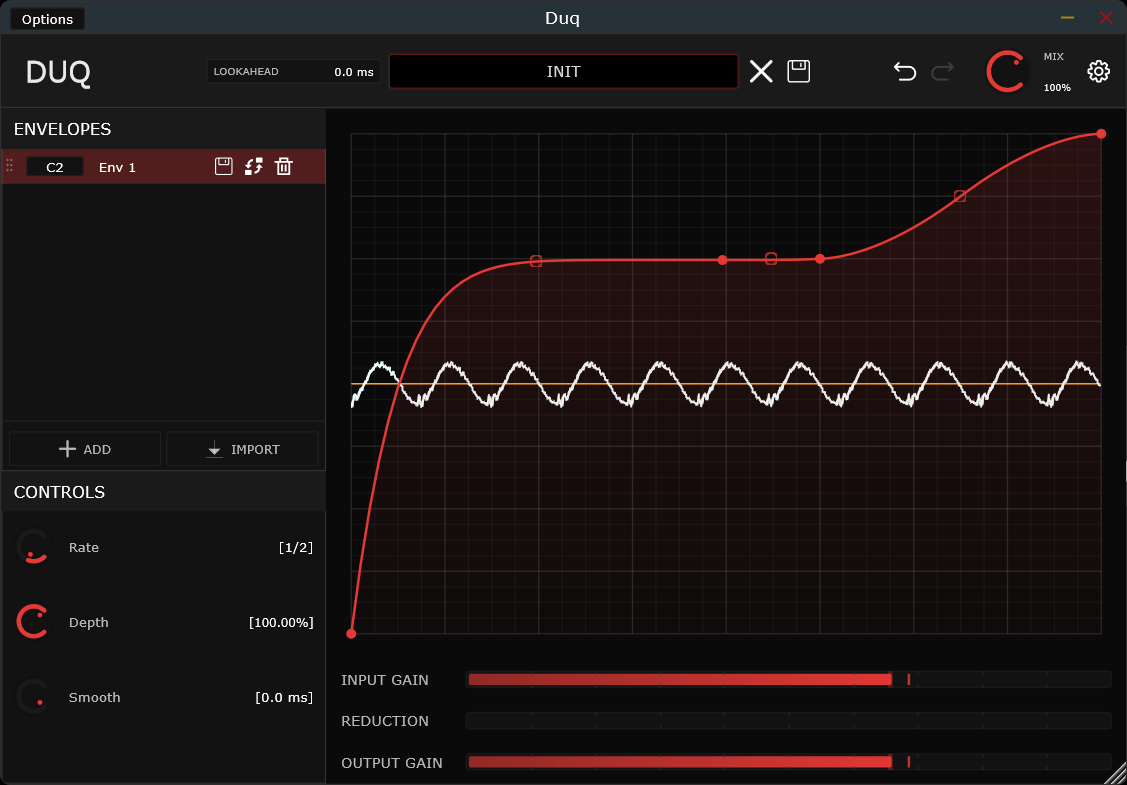
\includegraphics[width=0.8\textwidth]{figures/screenshot2.png}
    \caption{Envelope Modulation in Action}
    \label{fig:modulation}
\end{figure}
